\scanpage{24}
\mspage{5}
\figure{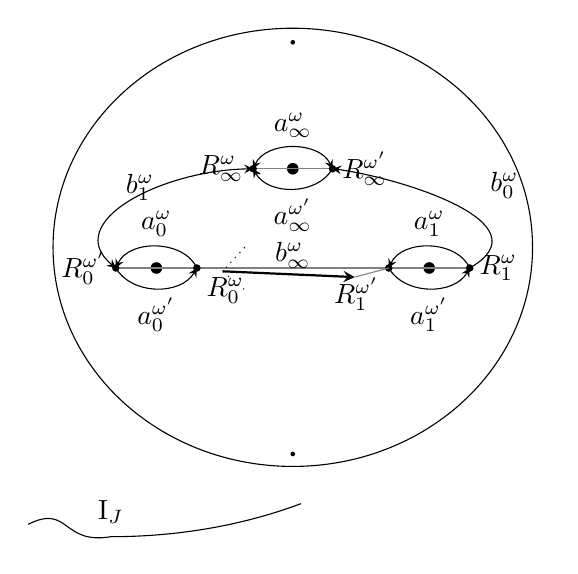
\begin{tikzpicture}[scale=1.05,>=stealth]
\draw[thin] (0,0) ellipse (2.9 and 2.65);
\fill (0,2.48) circle (.8pt);\fill (0,-2.5) circle (.8pt);
\fill (0,0.95) circle (2pt);\fill (-1.65,-0.25) circle (2pt);\fill (1.65,-0.25) circle (2pt);
\coordinate (ti) at (-.48,.95);\coordinate (tp) at (.48,.95);
\coordinate (li) at (-1.16,-.25);\coordinate (lp) at (-2.14,-.25);
\coordinate (ri) at (2.14,-.25);\coordinate (rp) at (1.16,-.25);
\draw[thin,gray] (ti)--(tp);\draw[thin,gray] (lp)--(ri);
\foreach \p in {ti,tp,li,lp,ri,rp}{\fill (\p) circle (1.3pt);}
\draw[<->] (ti) to[bend left=65] node[above] {$a_\infty^\omega$} (tp);
\draw[->] (tp) to[bend left=60] node[below] {$a_\infty^{\omega'}$} (ti);
\draw[->] (li) to[bend right=65] node[above] {$a_0^\omega$} (lp);
\draw[->] (lp) to[bend right=60] node[below] {$a_0^{\omega'}$} (li);
\draw[->] (ri) to[bend right=65] node[above] {$a_1^\omega$} (rp);
\draw[->] (rp) to[bend right=60] node[below] {$a_1^{\omega'}$} (ri);
\draw[<->] (ti) .. controls (-1.6,.93) and (-2.8,.30) .. (lp);
\node at (-1.85,.72) {$b_1^\omega$};
\draw[->] (ri) .. controls (3.1,.3) and (1.25,.85) .. (tp);
\node at (2.56,.75) {$b_0^\omega$};
\draw[dotted] (-.58,0)--(-.85,-.29)--(-.55,-.54);\draw[->,thick] (-.85,-.29)--(.75,-.36);
\draw[thin,gray] (.75,-.36)--(rp);\node at (0,-.10) {$b_\infty^\omega$};
\node[left] at (ti) {$R_\infty^\omega$};\node[right] at (tp) {$R_\infty^{\omega'}$};
\node[left] at (lp) {$R_0^{\omega'}$};\node[below right] at (li) {$R_0^\omega$};
\node[below left] at (rp) {$R_1^{\omega'}$};\node[right] at (ri) {$R_1^\omega$};
\node at (-2.2,-3.2) {$\mathrm I_J$};
\draw (-3.2,-3.35) .. controls (-2.7,-3.1) and (-2.8,-3.6) .. (-2.2,-3.5) .. controls (-1.1,-3.5) and (-.3,-3.25) .. (.1,-3.1);
\end{tikzpicture}}
$\unsure{\mathcal G_J|G_J}$ permute transitivement les six flèches $a_i^\omega$ et les six flèches $b_i^\omega$ : \deleted{$\unsure{Q|R}$}
\[
(1)\quad\left\{\begin{aligned}
a_i^\omega &: R_i^\omega\mathbin{-}R_i^{\omega'}\\
b_i^\omega &: R_{\omega i}^\omega\longrightarrow R_{\omega'i}^{\omega'}
\end{aligned}\right.
\]
\[
(2)\quad\left\{\begin{aligned}
\mathrm a)\quad &b_i^\omega b_i^{\omega'}=1&&\text{(trois relations effectives)}\\
\mathrm b)\quad &a_i^\omega b_{\omega'i}^{\omega}a_i^{\omega'}b_{\omega i}^{\omega}
a_{\unsure{\omega'i|\omega i}}^{\omega'}b_i^\omega=1&&\text{(deux relations effectives, une pour chaque }\omega\in\uline{\omega}\text{)}
\end{aligned}\right.
\]
\margin{\uline{NB}\quad $\tau(R_i^\omega)=R_i^\omega$\quad $\tau(a_i^\omega)=(a_i^{\omega'})^{-1}$\quad $\tau(b_i^\omega)=b_i^\omega$.}
\[
(3)\quad a_i^{\omega'}a_i^\omega=\lambda_i^\omega=\varphi_i^\omega(l_0)
\]
\[
(4)\quad \varphi_i^\omega:\quad
\Pi_{03}=\Pi_1(\unsure{U_{0,3}|\mathbf U_{0,3}};R_0^+)=\{l_0,l_1,l_\infty\mid l_\infty l_1l_0=1\}
\subset\widetilde\Pi_{0,3}=\Pi_1(\unsure{U_{0,3}|\mathbf U_{0,3}},\unsure{\mathcal G_J|G_J} R_0^+\unsure{)}
\]
\diagram{\begin{tikzcd}[ampersand replacement=\&,column sep=large]
\Pi_{03}\arrow[r]\&\Pi_1(\Sigma^*,R_i^\omega)
\end{tikzcd}}
\[
\begin{aligned}
l_0&\longmapsto a_i^{\omega'}a_i^\omega\\
l_1&\longmapsto (\unsure{b_{\omega i}^\omega|b_\infty^\omega})^{-1}a_{\omega i}^{\omega}a_{\omega i}^{\omega'}b_i^\omega
\end{aligned}
\]
Les $\varphi_i^\omega$ sont \unsure{permutés} entre eux \unsure{par les|par des} \unsure{formules} simples \unsure{de} transition
\[
(5)\quad\tau\varphi_i^\omega(g)=\varphi_i^\omega(\tau_\infty(g))
\qquad\text{où}\quad\tau_\infty\in\widetilde\Pi_{0,3}
\qquad\left\{\begin{aligned}
\tau_\infty(l_0)&=l_0^{-1}\\
\tau_\infty(l_1)&=l_1^{-1}\\
\tau_\infty(l_\infty)&=l_0l_1=\operatorname{int}(l_0)l_\infty^{-1}
\end{aligned}\right.
\]
\[
(6)\quad\left\{\begin{aligned}
a_i^\omega(\varphi_i^\omega(g))&=\varphi_i^{\omega'}(\varepsilon_0(g))\\
b_i^\omega(\varphi_{\omega i}^\omega(g))&=\varphi_{\omega'i}^{\omega'}(\sigma_\infty(g))
\end{aligned}\right.
\qquad\varepsilon_0^2=l_0
\]
\[
\begin{aligned}
\sigma_\infty(l_0)\unsure{'}&=l_1\\
\sigma_\infty(l_1)&=l_0\\
\sigma_\infty(l_\infty)&=(l_0l_1)^{-1}=l_1^{-1}l_0^{-1}=\operatorname{int}(l_0)l_\infty
\end{aligned}
\]
\deleted{$\unsure{\widetilde b_{\omega'i}^\omega|\widetilde b_i^\omega}$}

On introduit
\[
(7)\quad\widetilde b_i^\omega=a_{\omega'i}^{\omega'}b_i^\omega:
R_{\omega i}^\omega\mathbin{-}R_{\omega'i}^\omega,
\]
donc (2b) s'écrit
\[
(8)\quad\widetilde b_{\omega^2i}^\omega\widetilde b_{\omega i}^\omega\widetilde b_i^\omega=1
\]
\margin{\uline{NB} L'ens des $\widetilde b_i^\omega$ n'est pas stable sous $\tau$ il faudrait donc \unsure{aussi} prendre les $\tau\widetilde b_i^\omega$}
On aura
\[
(9)\quad\widetilde b_i^\omega(\varphi_{\omega i}^\omega(g))=\varphi_{\omega'i}^\omega(\rho^{-1}(g))
\qquad\rho^{-1}=\varepsilon_0\sigma_\infty
\qquad\left\{\begin{aligned}
\rho(l_0)&=l_1\\
\rho(l_1)&=l_\infty\\
\rho(l_\infty)&=l_0
\end{aligned}\right.
\]
Les relations 2(b) deviennent
\[
(\unsure{10})\quad\widetilde b_{\omega^2i}\widetilde b_{\omega i}\widetilde b_i=1
\]
\margin{23}
